\section{Methods}
\label{sec:method}

Both models can be seen in Figure~\ref{fig:methods:models}.
In the following, the three models we have developed, the networks they use as well as their cost functions are described.

\begin{figure*}
	\centering
	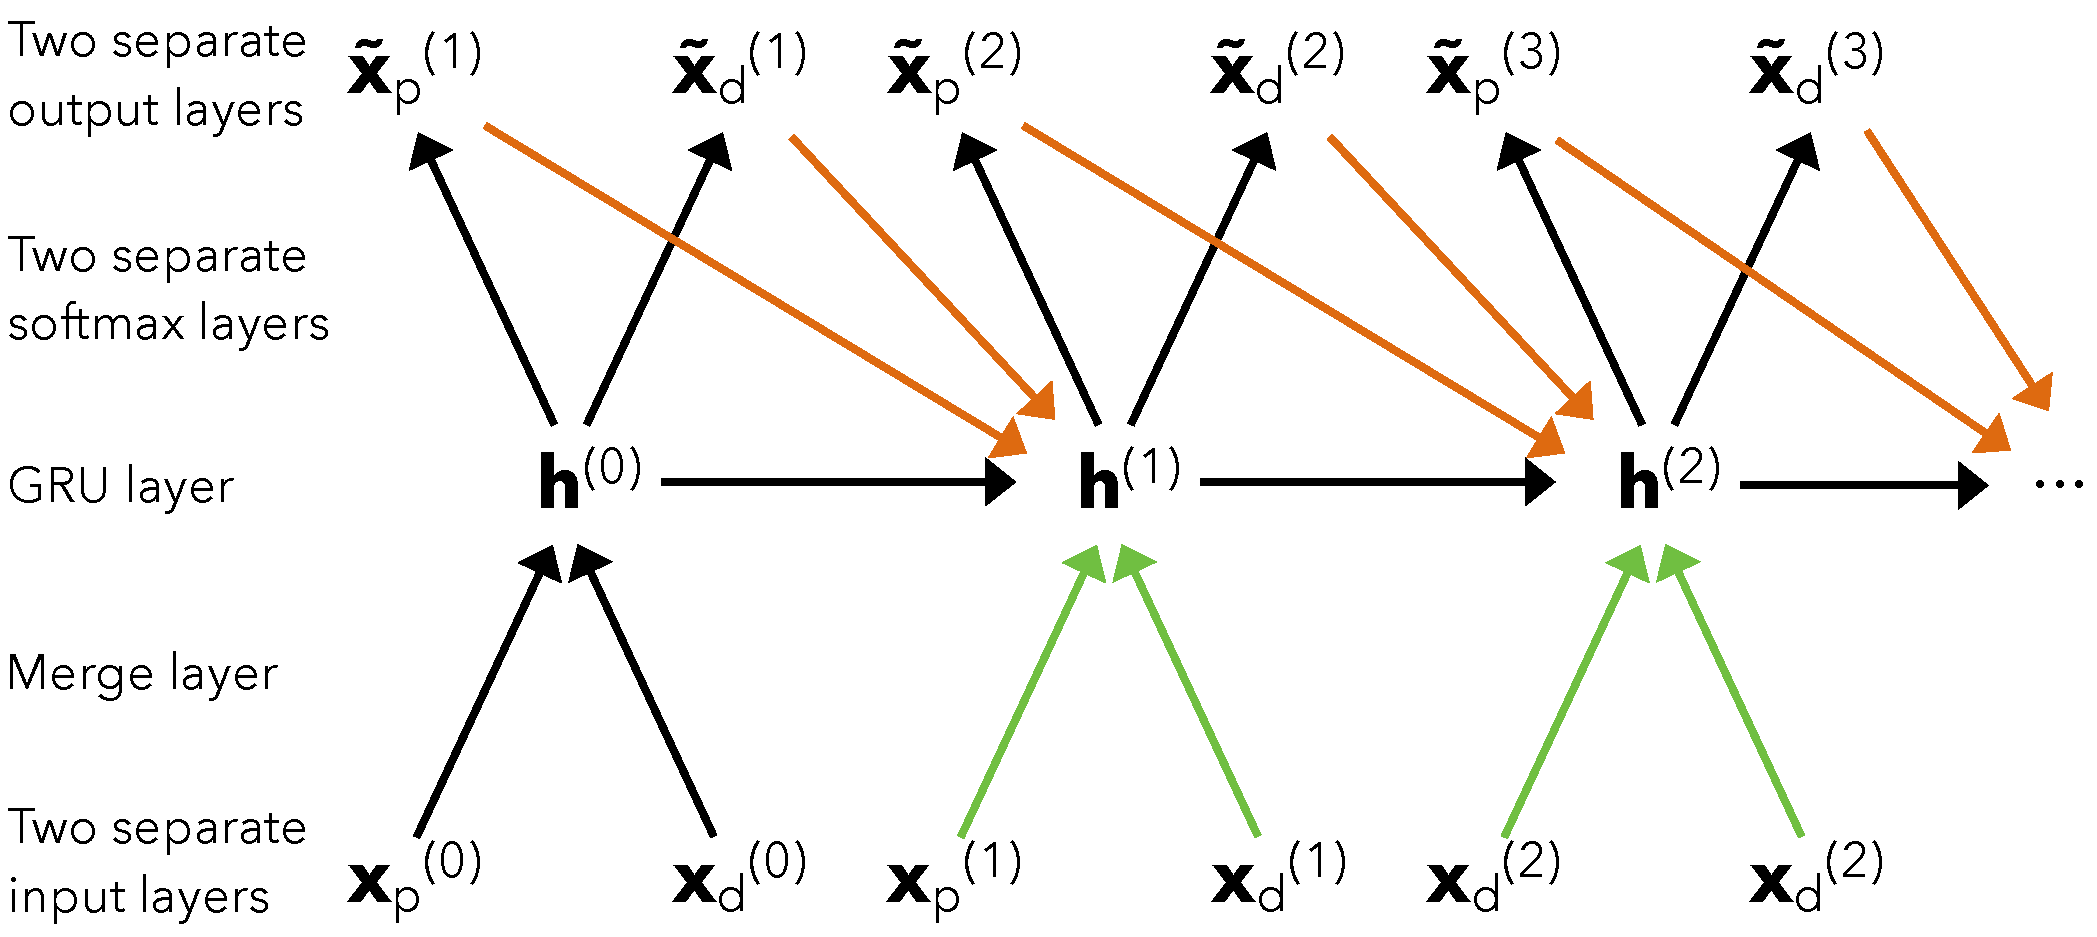
\includegraphics[width=0.6\textwidth]{Models}
	\caption{The setup for both models. $\vec{x}\order{t}\idx{p}$ and $\vec{x}\order{t}\idx{d}$ are the one-hot encoded pitch and duration, respectively, at position $t + 1$ in each sequence. The black arrows represent connections in all models, orange arrows represent connections present in models~2 and~3, and green arrows represent connections which are ignored in model~3.}
	\label{fig:methods:models}
\end{figure*}

\subsection{Conditional Distribution} % (fold)
\label{sub:conditional_distribution}
	The pitch $\vec{x}\order{t}\idx{p}$ and duration classes $\vec{x}\order{t}\idx{d}$ at step $t$ in a melody sequence, can be denoted by the combined feature vector $\vec{x}\order{t}=\set{\vec{x}\order{t}\idx{p},\vec{x}\order{t}\idx{d}}$.	
	The architecture of the full network model is based on the assumption of each note in the melody conditioning on all previous, so the next-step prediction of the network can be written as two conditional distribution:
	\begin{gather}
		\begin{split}
		\MoveEqLeft[3]
				p\left(\vec{x}\order{t+1}\idx{p}|\vec{x}\order{t'\le t}\right) \\ 
				& = p\left(\vec{x}\order{0}\idx{p}\right) \prod^{t+1}_{t'=1} p\left(\vec{x}\order{t'}\idx{p}|\vec{x}\order{t'-1}\right) \label{}
		\end{split} 	
	\end{gather}
	where the conditional distribution is similar for the duration classes.
% subsection conditional_distribution (end)

\subsection{Input network} % (fold)
\label{sub:input_network}
The input network merges the two one-hot-encoded class vectors into the two-hot-encoded vector, $\vec{x}\order{t}$. The input network also provides the binary mask for each melody for the network, so empty predictions are made when reaching the end of each melody, when the values in the mask becomes zero.
% subsection input_network (end)

\subsection{Recurrent neural network} % (fold)
\label{sub:recurrent_neural_network}
	The main part of the models is the recurrent neural network in the centre transferring temporal information from the input network to the output network.
	To enhance the long term memory, gated recurrent units (GRUs) are used. These are receiving $\vec{x}\order{t}$ for each step, $t$, in the melody. Each GRU run through the melody step by step, as in \cite{Chung2014}, calculating the hidden activations recursively by the activation functions:
	\begin{alignat}{2}
	 	& \text{Reset:} \; & \vec{r}\order{t} &= \sigma_r\left(\vec{x}\order{t} \mat{W}_{xr} + \vec{h}\order{t-1} \mat{W}_{hr} + \vec{b}_r\right) \label{gru:reset} \\
        & \text{Update:} \; & \vec{u}\order{t} &= \sigma_u\left(\vec{x}\order{t} \mat{W}_{xu} + \vec{h}\order{t-1} \mat{W}_{hu} + \vec{b}_u\right) \label{gru:update} \\
        & \text{Candidate:} \; & \vec{c}\order{t} &= \sigma_c\left(\vec{x}\order{t} \mat{W}_{xc} + \vec{r}\order{t} \odot \left(\vec{h}\order{t-1} \mat{W}_{hc}\right) + \vec{b}_c\right) \label{gru:candidate} \\
        & \text{Activation:} \; & \vec{h}\order{t} &= \left(1 - \vec{u}\order{t}\right) \odot \vec{h}\order{t-1} + \vec{u}\order{t} \odot \vec{c}\order{t} \label{gru:activation}
	\end{alignat}
	where $\mat{W}_x$ are the vertical weights transforming the current input $\vec{x}\order{t}$ linearly and the $\mat{W}_h$ are the horizontal weights transforming the previous activation linearly, so information about previous states can propagate horizontally through each step. The non-linear sigmoid functions are the logistic function ($\sigma(\vec{x})=(1+\eup^{-\vec{x}})^{-1}$) for the reset gate in equation~\eqref{gru:reset} and update gate in equation~\eqref{gru:update} and the hyperbolic tangent function for the candidate activation in equation~\eqref{gru:candidate}. The reset gate controls how much of the signal from the previous activation, $\vec{h}\order{t-1}$, will be a part of the current candidate activation, $\vec{c}\order{t}$, in equation~\eqref{gru:candidate} and the update gate then controls the proportional mixing of $\vec{h}\order{t-1}$ and $\vec{c}\order{t}$ in the new activation, $\vec{h}\order{t}$, in equation~\eqref{gru:activation}. This means that $(\vec{r}\order{t}, \vec{u}\order{t}) = (0,1)$ will cut off the signal from the previous states and $(\vec{r}\order{t}, \vec{u}\order{t}) = (1,0)$ will copy the previous activation entirely. This makes it possible for the model to condition the next prediction over long terms, like the overall tonality and common motifs, and short terms, like previous pitch interval jumps and current harmony (chords). The models ability to perform this temporal conditioning in a musical manner is what will be investigated in the experiment section. 

	When computing the back-propagation through time for adjusting the model parameters in recurrent neural networks, vanishing gradients can be a huge problem leading to premature convergence (stopped learning). This is due to neurones in the network being saturated, when the gradient of the activation function is close to zero near convergence along the tails. The gradients will therefore vanish after multiple multiplication in the back-propagation, where each gradient depends on the previous. 
	Exploding gradients can also occur when training recurrent neural networks, so a gradient clipping of $3$ is used for all gradients.  
% subsection recurrent_neural_network (end)

\subsection{Output network} % (fold)
\label{sub:output_network}
	The output network consists of two standard feedforward neural networks with softmax activation functions for class probabilities. A neurones response to the hidden GRU states at time $t$ represents the probability of the next note at time $t+1$ belonging to a specific pitch class for the pitch network and duration class for the duration network.
	The conditional probability for pitch class $p$ at time $t+1$ is then given by the output network as:
	\begin{equation}
		p\left(\tilde{\vec{x}}\order{t+1}\idx{p}|\vec{x}\order{t'\le t}\right) = s\left(\mat{W}\idx{p} \vec{h}\order{t} + \vec{b}\right)%\frac{\eup^{\vec{h}\order{t}}}{\sum^K_{k=1}}
	\end{equation}
	where $s(\vec{x})$ is the softmax activation function and the same holds for duration classes. 

	% As $\vec{h}\order{t}$ is a non-linear function of all previous notes $\vec{x}\order{t'<t}$ indirectly through the previous activation $\vec{h}\order{t-1}$ and of the current note $\vec{x}\order{t}$ directly through the input network.   
	
	\subsection{Extended model} % (fold)
	\label{sub:extended_model}
	By plugging in the next-step prediction of the output network to the next step input of the GRU layer an extra loop is formed which transfers additional information about the previous step and penalises the model more for prediction errors.  
	Adding the most probable prediction $\tilde{\vec{x}}\order{t}$ from previous step to the original input, $\vec{x}\order{t}$ after weighting and transforming both through a ReLU dense layer will combine the new input $\hat{\vec{x}}\order{t}$, which will go into the activation functions in Equation~\eqref{gru:reset}-\eqref{gru:activation} in the exact same manner. This model is also referred to as model 2 and the normal model as model 1.
	
	The only difference between the two models is the usage of the previous output, so if a wrong prediction in the previous output leads to higher misclassification in the next step an avalanche of misclassifications roll along the sequence. So during training the model would gain the lowest cost by just lowering the connection throughput of the previous output and finally reduce model 2 to model 1.
	To avoid this a third model without any original input, except the first note to kickstart it has also been implemented.
	% subsection extended_model (end)

	\subsection{Cost function} 
	The categorical cross entropy cost function for example $n$ is:
	\begin{equation}
		%L(\vec{x}\order{t}; \vec{f}) = \frac{1}{T}\sum^{T-1}_{t} \sum^{M}_{m} \left(\vec{x}_{m}\order{t+1} \log f(\vec{x}\order{t}) + \log(1-f(\vec{x}\order{t})  \right)
		L_n = -\sum^{T-1}_{t}\sum^{K}_{k} \vec{x}\order{t+1}\idx{k} \log p\left(\tilde{\vec{x}}\order{t+1}\idx{k}|\vec{x}\order{t'\le t}\right)
	\end{equation}
	summed over all $K$ classes and time steps except the last one, $T$. All time steps are treated as separate data points, so the targets and outputs are unrolled and the loss for each are averaged over the examples, $n$, in the mini-batch, after masking out the steps outside the melodies. 

% subsection output_network (end)


% \subsection*{EHR synopsis}

% To apply the Deepr model to the EHR data, we will be working with text preprocessing methods, like one-hot encoding and word-embedding, on irregular time-series of diagnosis codes converted into sentences with time intervals between hospital visits inserted as special words (e.g., “1--3m” for 1 to 3 months). Therefore this task is comparable to applying convolutional neural networks (CNNs) for natural language processing problems, looking for local patterns and summing these up to a global classification.

% The Doctor AI paper’s model is implemented using multi-hot encoding of all diagnoses and medications recorded at each hospital visit with a timestamp. A two-layer recurrent neural network (RNN) are used for predicting diagnoses given at and durations between future hospital visits. The predictive power of this model lies in its ability to connect diagnoses in long term patterns important to future diagnoses.

% We will investigate the possibilities of using dilated causal convolutions as a cross between the CNN and RNN methods for predicting future diagnoses. Google DeepMind use these convolutions for predicting future audio samples in speech synthesis with WaveNet.

% A. van den Oord et al.: “WaveNet: A Generative Model for Raw Audio”, September 2016.
